\documentclass{bioinfo}
\usepackage[english]{babel}
\copyrightyear{2015} \pubyear{2015}
\usepackage{natbib}
\bibliographystyle{natbib.bst}


\access{Advance Access Publication Date: Day Month Year}
\appnotes{Manuscript Category}

\renewcommand{\cite}{\citep}
\usepackage{todonotes}

\begin{document}
\firstpage{1}

\subtitle{Subject Section}
\newcommand{\name}{Voodoo }

\title[short Title]{\name: Combining Bottom-up and top-down approaches through graph learning over interaction networks for drug-target-interaction prediction}
\author[Sample \textit{et~al}.]{Tilman Hinnerichs\,$^{\text{\sfb 1,}*}$ and Robert Hoehndorf\,$^{\text{\sfb 2}}$}
\address{$^{\text{\sf 1}}$Department, Institution, City, Post Code, Country and \\
$^{\text{\sf 2}}$Department, Institution, City, Post Code,
Country.}

\corresp{$^\ast$To whom correspondence should be addressed.}

\history{Received on XXXXX; revised on XXXXX; accepted on XXXXX}

\editor{Associate Editor: XXXXXXX}

\abstract{\textbf{Motivation:} Text Text Text Text Text Text Text Text Text Text Text Text Text
Text Text Text Text Text Text Text Text Text Text Text Text Text Text Text Text Text Text Text
Text Text Text Text Text Text Text Text Text Text Text Text Text Text Text Text Text Text Text
Text Text Text Text Text Text
Text Text Text Text Text.\\
\textbf{Results:} Text  Text Text Text Text Text Text Text Text Text  Text Text Text Text Text
Text Text Text Text Text Text Text Text Text Text Text Text Text  Text Text Text Text Text Text\\
\textbf{Availability:} Text  Text Text Text Text Text Text Text Text Text  Text Text Text Text
Text Text Text Text Text Text Text Text Text Text Text Text Text Text  Text\\
\textbf{Contact:} \href{tilman.hinnerichs@kaust.edu.sa}{tilman.hinnerichs@kaust.edu.sa}\\
\textbf{Supplementary information:}10264703 Supplementary data are available at \textit{Bioinformatics}
online.}

\maketitle
\section{Introduction}

\cite{Survey2018}\\
In history, traditional remedies, that were known for their medicinal
properties lead to drugs by extraction of the functional
ingredients. Alternatively, characteristics and features of potential
drugs were detected by accident like in the case of penicillin. More
recently, biological drug targets can be found \textit{in silico}
through discovery of suitable computational predictors.


The challenge of accurately predicting drug-target-interactions (DTI)
has shown its importance in the fields of drug repurposing and
repositioning, and in the exploration of novel drugs and their
interaction partners. Knowledge about those links between compounds
and their target proteins help in an array of medical and
pharmaceutical studies. Additionally, those associations can be
utilized to identify disease specific targets, leading to desirable
therapeutic effects.

With the rapidly growing field of machine learning approaches and
their application to bioscientifical problems in the realm of
bioinformatics, different kinds of data, such as long DNA sequences
could be utilized for feature generation, while rapid advances were
made. Almost all state of the art models for drug-target-interaction
prediction were based on the usage of neural networks with increasing
size.\todo{Needs ref, or reformulate}

Only recently, the technique of graph learning was introduced by
\citet{GCNConv} through graph convolution algorithms, and improved and
altered under usage of different kernels \cite{ChebConv, ARMAConv},
attention mechanisms \cite{GATConv}, random walks \cite{APPNPConv},
and mixtures of both \cite{SAGEConv}. While based on diverse systems,
they can be relevant for testing distinct hypothesis for given
graphs. While convolutional filters are suitable for finding patterns
among the the given graph, attention mechanisms are more relevant for
discovery of important regions within. Lately, graph learning
approaches found application for computing compound representations
for DTI prediction.

Approaches on this rather sophisticated\todo{Try to avoid}
problem\todo{Need to state the problem clearly here or at end of prev
  paragraph} can divided into top-down or network approaches
(\textbf{CITATION}), and bottom-up or molecular approaches
(\textbf{CITATION}). Top-down approaches take advantage of other data
such as diseases (CITATION), side effects, knowledge graphs or
ontologies, in order to learn representations for both compound and
protein. \todo[inline]{We call these approaches ``top-down'' because
  they start with the observable characteristics induced by a drug and
  infer the targets based on the likely molecular mechanisms that
  result in these phenotypes.} On the other hand, bottom-up approaches
attempt to learn from chemical properties of proteins or drugs to
infer candidate drug--target interactions. For drugs, molecular
structure (CITATION GraphDTA), molecular fingerprints, similarity to
other drugs (See Bioinf Survey), and other molecular features may be
used. On the protein side, secondary structure prediction (CITATION),
contact prediction (CITATION), or simply\todo{Don't use ``simply''.}
convolution over the amino acid sequences can be used to obtain a
feature representation for a given proteins. However, both bottom-up
and top-down approaches to drug--target interaction prediction
\todo[inline]{replace: ``contain and share some problems'' with
  something like ``have some limitations''} that are not solvable within
themselves.
\todo[inline]{Following is not sufficiently precise; here, you need to
clearly state the challenges faced by both approaches, ideally with
references.}
Thus, bottom-up approaches share the lack of ability to
generalize, which we will show in later sections, and usually focus on
engineering sophisticated features for the drugs, while neglecting to
formulate meaningful features on the protein side. Top-down approaches
lack the ability to spot small differences to cope with small
differences within the drug structure and rely heavily on given data
for the considered drug-target pair. The latter is not suitable for
predictions on novel or unseen compounds, as e.g., data on side
effects or its impact on diseases is seldom given for novel drugs.

In order to design such a feature for proteins and drugs,
respectively, we make use of the interaction networks for both
proteins and compounds. Drug-drug interaction networks were introduced
and standardized by \citet{Boyce2015} and have been used for clinical
decision support \cite{Scheife2015}. Drug-drug interaction networks
may give a hint on common targeted pathways. As an additional compound
feature we will use semantic side effect similarity, which we will
discuss later on\todo{Generally, try to avoid pointers to ``later''.}.

Protein-protein interaction networks have shown great results in
$\dots$(\cite{Vazquez2003}, \cite{Ackerman2019}) in granting context
for molecular system biology. However, these contexts were never
applied to the problem of drug-target-interaction prediction. Thus we
formalized our hypotheses over these interaction graphs and will test
them in the following chapters.

\enlargethispage{12pt}

\section{Methods}
\subsection{Problem Description}
The issue of predicting drug-target interactions can be described
quite briefly: For a given drug and a given protein we want to
determine whether those interact or not.  We do not differentiate
between types of interaction such as activation and inhibition, and do
not predict the strength of the interaction.  If we additionally make
the closed world assumption, i.e., assume that our knowledge is
complete and all drug--protein pairs without a known interaction do
not interact, we can formulate the problem as a binary classification
task.


\subsection{Datasets}
We obtain a dataset consisting of $\approx 11000$\todo{precise number}
human proteins with over 170.000\todo{exact number} links from STRING
\citep{STRINGv10}. For the drug-target interactions, we
fetched 137,000\todo{precise} links from the STITCH database
\citep{STITCHv5}. As both STRING and STITCH provide confidence scores
for each association, we filtered them as advised by a threshold of
$700$, therefore retaining only high-confidence interactions.

We utilize the PhenomeNET ontology \citep{PhenomeNET2011}, an ontology
integrating ontologies such as the Human Phenotype Ontology
\citep{HPO2018}, Gene Ontology \cite{GOoriginal2000, GOrecent2020},
Mammalian Phenotype Ontology \citep{MP2009} and several others.
We obtained side effects and their links to drugs from SIDER
\citep{SIDER}; SIDER contains side effects encoded using identifiers
from the MedDRA database \citep{MedDRA}. We mapped side effects to the
PhenomeNET ontology using the \textit{Phenomebrowser.net}, which
provides a SPARQL query endpoint for the mentioned resources.

We only use proteins in our analysis that have at least one link in
either STITCH or STRING, and drugs with at least one side effect and
one existing target. Therefore, the intersection between these
resources yields 1,160 drugs and 6,680 human proteins for the training
phase. We provide links to and methods for obtaining and processing
the necessary data on Github.

For comparative evaluation, we use the gold standard dataset
introduced by \citet{Yaminishi2008} \todo[inline]{consisting of XXXX
  interactions between XXX drugs and XXX protein targets}.
 
\subsection{Model}

Our model combines ``top-down'' and ``bottom-up'' information for
drug--target identification. We consider an approach to be
``top-down'' when observable characteristics of either a drug (such as
a drug effect) or protein (such as a protein function, or phenotypes
resulting from a loss of function) are used to provide information
about a molecular mechanisms; we consider an approach ``bottom-up''
when structural or other molecular information is used to determine a
mechanism.  In order to build a method that incorporates both top-down
and bottom-up features, we first create a model for each type of
feature separately.  As features for the bottom-up model, we use
features derived from molecular structures of drugs from the
\textit{SmilesTransformer} \citep{SmilesTransformer} and molecular
features for proteins from \textit{DeepGOPlus}
\citep{DeepGoPlus}. \textit{SmilesTransformer} introduces an
autoencoder, learning over the SMILES strings and therefore the
molecular organization of each drug in an unsupervised manner. 
\textit{DeepGOPlus} provides  features derived from protein amino acid
sequences which are useful to predict protein function.
% Thus, both embeddings seem to suitably supplement
% the following ontology based representations.

As phenotypes and functions are encoded through ontologies, we use
DL2Vec \citep{DL2vec2020} to obtain ontology based representations for
use as top-down features. DL2vec constructs a graph by introducing
nodes for each ontology class and edges for ontology axioms, followed
by random walks starting from each node in the graph. These walks are
encoded using a Word2vec \citep{Word2vec2013} model. Therefore, DL2Vec
generates representations that can encode drug effects or protein
functions while preserving their semantic neighbourhood within that
graph.

% The overall structure of the ontology can be seen in
% Figure~\ref{fig:Onto}.

\todo[inline]{Consider supplement, or combine with other figures.}
\begin{figure}[!tpb]%figure1
	\centerline{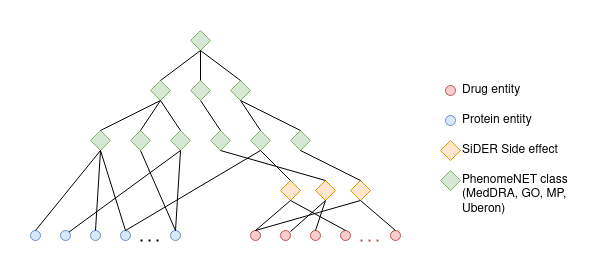
\includegraphics[width=0.5\textwidth]{figures/drug_protein_ontology_network.png}}
	\caption{Drugs and proteins with annotations to SiDER and PhenomeNET}
	\label{fig:Onto}
\end{figure}


\subsubsection{Siamese neural networks and modular learnable feature transformation}

\todo[inline]{Looking at the code, I wonder if what is implemented is
  actually a Siamese ANN; it does not look as if the weights are
  shared between the two networks, so looks more like a twin or
  half-twin network? Siamese would be sim(f(e1),f(e2)) but the
  implementation seems to be sim(f(e1), g(e2)).}

As we want to learn from the similarity of drug side effects and
protein phenotypes, we use a deep Siamese neural network with
a contrastive loss using cosine similarity.
A Siamese neural network aims to learn a similarity between two
embeddings.

% learning a high-dimensional embedding emphasizing this identity by
% forcing a similarity between these embeddings. On the other hand we
% built a deep neural network for the molecular structure based
% features, also benefiting from the siamese network
% architecture. Computing the similarity between two representations,
% allows for a variety of different methods.  
% However, we decided for
% the cosine similarity measure being invariant to scaling.

Therefore, the precomputed embeddings are run through a regular,
neural learnable feature transformation (LFT) network, which also
reduces the eventual representation size for drugs and proteins
separately. An example structure for both types of features can be
found in Figure~\ref{fig:SiameseNetwork}.

While a regular deep neural network, denoted by LFT, for feature space reduction is not particularly novel, we emphasize the versatility of this approach, as both ontology and molecular feature for both drugs and proteins are reduced to similar dimensionality. This allows for a high amount of modularity and different experimental setups by plugging different kinds of features into the model. Additionally, these pretrained features can be used for a variety of other tasks. Additionally, the ontology LFT can be reused for a variety of DL2vec based features with respect to other ontologies and hypotheses. We hereby followed the results of \textit{DL2vec}, indicating that utilizing the activation function $\sigma := \mathrm{LeakyReLU}$ leads to performance increase.



\begin{figure}[!tpb]%figure1
	\centerline{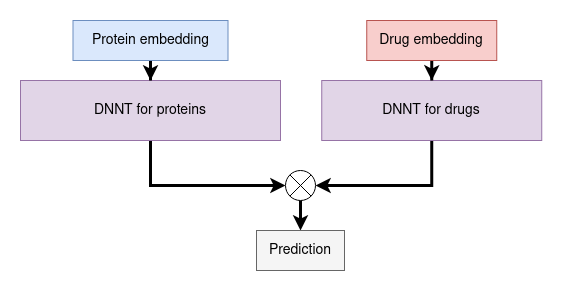
\includegraphics[width=0.35\textwidth]{figures/siamese_network.png}}
	\caption{Siamese network applied to molecular and DL2vec
          features, utilizing deep learnable feature transformations
          (LFT). The similarity function $\otimes$ yields the
          similarity between both transformed embeddings e.g. by
          computing the cosine similarity.}
	\label{fig:SiameseNetwork}
\end{figure}




\subsubsection{Graph convolutional layers}

We included these molecular and ontology-based sub-models with a
larger graph convolutional model. The graph underlying the graph
convolutional neural network is based on the protein--protein
interaction (PPI) graph. The PPI dataset is represented by a graph
$G=(V,E)$, where each protein is represented by a vertex $v\in V$, and
each edge $e\in E\subseteq V\times V$ symbolizes an interaction
between two proteins. Additionally, we introduce a mapping
$x:V\rightarrow\mathbb{R}^{d}$ projecting each vertex $v$ to its node
feature $x_v := x(v)$, where $d$ denotes the dimensionality of the node
features.
 
% As described before, graph convolution has shown significant
% performance increase in a variety of tasks. While there are various
% methods out there we will only introduce the most basic one here. 
A graph convolutional layer \citet{GCNConv} consists of a learnable
weight matrix followed by an aggregation step, formalized by
\begin{equation}
	\mathbf{X}^{\prime} = \mathbf{\hat{D}}^{-1/2} \mathbf{\hat{A}}
	\mathbf{\hat{D}}^{-1/2} \mathbf{X} \mathbf{\Theta}
\end{equation}
where for a given graph $G=(V,E)$, $\hat{A} = A + I$ denotes the
adjacency matrix with added self-loops for each vertex, $D$ is
described by $\hat{D}_{ii} = \sum_{j=0} \hat{A}_{ij}$, a diagonal
matrix displaying the degree of each node, and $\Theta$ denotes the
learnable weight matrix. Added self-loops enforce that each node
representation is directly dependent on its own preceding one. The
number of graph convolutional layers stacked equals the radius of
relevant nodes for each vertex within the graph.

The update rule for each individual node is
\begin{equation}
	\mathbf{x}^{\prime}_i = \mathbf{\Theta} \sum^{N}_{j}
	\frac{1}{\sqrt{\hat{d}_j \hat{d}_i}} \mathbf{x}_j
\end{equation}
where both $\hat{d}_i, \hat{d}_j$ are dependent on the edge weights
$e_{ij}$ of the graph. With simple, single-valued edge weights such as
$e_{ij}=1 \text{ }\forall (i,j)\in E$, all $\hat{d}_i$ reduce to
$d_i$, i.e., the degree of each vertex $i$. We denote this type of
graph convolutional neural layers with \textsc{GCNConv}.

While in this initial formulation the node-wise update step is defined
by the sum over all neighbouring node representations, we are able to
alter this formulation to another message passing scheme.  We are able
to rearrange the order of activation function $\sigma$, aggregation
$\mathrm{AGG}$ and linear neural layer $\mathrm{MLP}$ with this
formulation as proposed by \citet{GENConv2020}:
\begin{equation}
	\mathbf{x}_i^{\prime} = \mathrm{MLP} \left( \mathbf{x}_i +
	\mathrm{AGG} \left( \left\{
	\mathrm{\sigma} \left( \mathbf{x}_j + \mathbf{e_{ji}} \right) +\epsilon
	: j \in \mathcal{N}(i) \right\} \right)
	\right)
\end{equation}
where we will generally only consider
$\sigma \in \{\mathrm{ReLU}, \mathrm{LeakyReLU}\}$. We will denote
this generalized layer type as \textsc{GENConv}, following the
notation of PyTorch Geometric \cite{PytorchGeometric}.  While the
reordering is mainly import for numerical stability, this alteration
also addresses the vanishing gradient problem for deeper convolutional
networks \cite{GENConv2020}. Additionally, we can also generalize the
aggregation function to allow different weighting functions such as
learnable $\mathrm{SoftMax}$ or $\mathrm{Power}$ for the incoming
signals for each vertex, substituting the averaging step in
\textsc{GCNConv}. Hence, while \textsc{GCNConv} suffers from both
vanishing gradients and signal fading for large scale, highly
connected graphs, each propagation step in \textsc{GENConv} emphasizes
signals with values close to $0$ and $1$. The same convolutional
filter and weight matrix are applied to and learned for all nodes
simultaneously. % , and the resulting information\todo{Which information?
  % Specify} hold no information on their own connectivity.
We further employ another mechanism to avoid redundancy and fading
signals in stacked graph convolutional networks, using residual
connections and a normalization scheme \cite{DeepGCN2019,
  DeeperGCN2020}.
The residual blocks are reusable and can be stacked multiple times. %, thereby not losing focus of each node neighbourhood.
\todo[inline]{Needs a clearer outline/description/figure of YOUR model
structure.}
The structure is depicted in Figure~\ref{fig:ResGraphConvBlocks}.

\begin{figure}[!tpb]%figure1
	\centerline{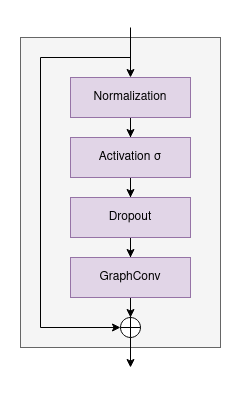
\includegraphics[width=0.5\columnwidth]{figures/ResGraphConvBlocks.png}}
	\caption{Residual architecture built by \citet{DeepGCN2019} and \citet{DeeperGCN2020} enabling deeper graph convolutional models}
	\label{fig:ResGraphConvBlocks}
\end{figure}




\subsubsection{Hyperparameter tuning}
As the number of drug-targets are sparse with respect to the number of
both drugs and proteins considered, the training, validation and
testing datasets are imbalanced. As there are only $22,336$ links in
the considered subset the ratio
\begin{equation*}
	\frac{\#drugs \cdot \#proteins}{\#dti\_links} \approx 360,
\end{equation*}
consequently needing compensation in the computed loss function and
appropriate metrics for the evaluation.

Therefore, we weighted all positive drug-protein pair samples with
this ratio by introducing the following loss function with respect to
binary cross-entropy:
\begin{equation}
	l(x,y) = - w \left[ y \cdot \log x + (1 - y) \cdot \log (1 - x) \right]
\end{equation}
for a given prediction $x$ and target $y$. We average this loss among
all drug-protein pairs in the training set, leading to a stable
environment for the used optimizing scheme \textit{Adam}
\citep{Adam2014}. We implemented a 5-fold cross validation among the
proteins. Furthermore, we used early stopping to detect plateaus in
the training process.

To find the best hyperparameter configuration for the proposed model
we performed a grid search to find the most expressive and
non-redundant representation. We pretrained the bottom-up and the
top-down model separately and aimed at best performing models
with respect to our evaluation metrics. We optimized embedding sizes,
depth of the neural network, optimizer, learning rate and layer types
using an extensive, manual grid search. \todo[inline]{Specify range of
  values searched here; even better if you have the intermediate
  results and can put them here (better: in the supplement).}

\subsection{Evaluation and metrics}

To assess each model, we compute a variety of common metrics for
binary classification. As the datasets are highly imbalanced, we use
the area under the receiver operating characteristic curve
(AUROC) on training, validation and testing split. % We
% calculated the true positive rate (TPR), false positive rate (FPR), and
% precision score. We will further compute true positives (TP), false
% positives (FP), false negatives (FN) and finally true negatives (TN).

\todo[inline]{Needs a statement on how the PAIRS are ranked here and
  TPR/FPR is calculated based on the ranks of the DT-PAIRS.}
We calculate the AUROC by computing true positive rate at various
false positive rate thresholds and using trapezoidal approximations to
estimate the area under the curve. We refer to this measure as
$MacroAUC$.

\todo[inline]{For RH: check this again later:}
In contrast we also calculate the $MicroAUC$ score. For given lists $D, P$ of drugs and proteins, respectively, and a set of known interactions $Int := \{(d_i, p_i) \}$, \textit{MicroAUC} is calculated as the average per entity (macro) \textit{AUROC} score. With respect to proteins, this can be formalized for given labels and prediction $l,y:D\times P \rightarrow \{0,1\}$  as 
\begin{equation*}
	MicroAUC_p := \underset{p\in P}{mean}\left(\left\{ \text{AUROC}(\{ (l(d_i, p), y(d_i,p))| d_i\in D\}) \right\}\right)
\end{equation*}

Drugs and proteins can be interchanged in this formulation, and we
refer to the different measures as a protein-centric microAUC
($MicroAUC_p$) and a drug-centric microAUC
($MicroAUC_d$). Additionally, the $MicroAUC$ score may not be defined
as, in some datasets some targets or drugs, respectively, do not have
any interactions, leading to an infeasible $TPR$ and an undefined
$AUROC$ score for that entity.
\todo[inline]{Don't understand this, can you add the formula:} For
those entities we impute the $MicroAUC$ linearly, by using the
accuracy for this subset.



\section{Results}

\subsection{\name: computational model to identify drugs that target a
  protein}

% As in machine learning inference is derived from the underlying data,
% models and data are naturally and intrinsically linked. Thus, the more
% we understand about the pitfalls and biases within the data, the more
% we can try to bypass these difficulties. We will hereby abbreviate,
% e.g., a cross validation splitting scheme as \glqq split\grqq{}
% determining the train, validation and test subset of a given dataset.

Within DTI prediction, there are potential biases resulting from the
underlying datasets \citep{Pahikkala2014}. First, novel drugs are
often designed by altering non-functional components of a drug,
leading to two and more very similar drugs designed to target the same
proteins \cite{Overington2006}. This can result in a bias when it
leads to hidden duplicates that can distribute among the train/test
split, resulting in a better (measured) predictive performance than
would be expected when the model is applied to identify drugs that
target a protein for which no drugs yet exist. Second, some proteins
(which we will denote as \textit{hub proteins}) have significantly
more known interactions with drugs than others. In the STITCH
database, $5\%$ of the proteins have $40\%$ of the interactions, and
similar distributions are present in the Yamanishi and Drugbank
datasets \cite{Drugbank2007, Drugbank2017} datasets; preferentially
predicting these proteins may increase predictive performance while
again not reflecting the actual performance when applied to a new
protein (e.g., a protein for which no interactions are known). These
differences in the number of drugs targeting certain proteins may be
the result of study bias where more ``valuable'' proteins have more
drugs designed to target them due to their involvement in more common
diseases (or diseases for which drugs can be more profitably
marketed).

We developed \name as a computational model to predict drug--target
interactions. Specifically, given a protein, \name will identify and
rank known drugs that likely target this protein. \name combines two
types of features: structural information for drugs and proteins that
can be used to determine if they may physically interact, and
information about drug effects that may localize on an interaction
network.  As structural features, \name uses structural
representations of drugs from the SMILES transformer
\cite{SmilesTransformer} and representations of protein amino acid
sequences from DeepGOPlus \cite{DeepGoPlus}.  \name learns
representations of drug effects and protein functions using the
ontology-based machine learning method DL2Vec \cite{DL2vec2020}.

\todo[inline]{Move to methods:}
When combining ontology and molecular features with or without the
graph model, we concatenate both protein features and both drugs
features, before plugging them into the graph or the similarity
computation.

We use two Siamese neural networks to combine the molecular and
phenotype representations of drugs and proteins, and add these to a
protein interaction network as node labels.  We then train this model
in an end-to-end manner using a graph neural network architecture.
The overall workflow\todo{make sure it's a workflow} is depicted in
Figure~\ref{fig:Fullmodel}.


% Note that this approach can be easily generalized, profiting from
% other protein function and phenotype representation methods.


\begin{figure}[!tpb]
	\centerline{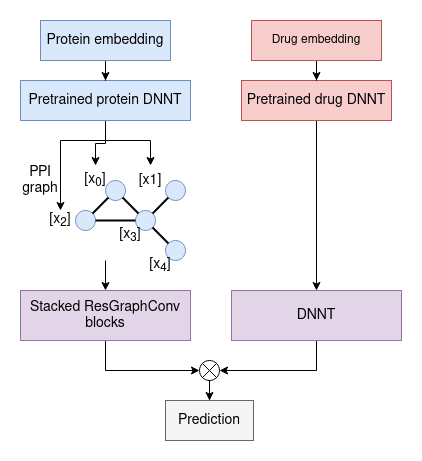
\includegraphics[width=0.45\textwidth]{figures/full_model.png}}
	\caption{Full DTI prediction model based on the pretrained learnable feature transformations (LFT) for either molecular structure or ontology based features. The transformed protein representations are added to each corresponded protein as node features for the graph convolutional steps. }
	\label{fig:Fullmodel}
\end{figure}

Through the very nature of the graph convolutional neural network, we build the transformed representation for all proteins in every forwarding step of the model. Note particularly, that the same convolutional filter and weight matrix are applied to and learned for all nodes simultaneously. By construction, for a single drug we can compute and predict all its interactors in a single run of the model, leading to significantly less computing time. 



\subsection{\name identifies drugs that target a protein}

\todo[inline]{Likely discussion:}
The aim of \name is to predict candidate drugs that target a given
protein; the challenge is to develop a training and evaluation scheme
that does not simply overfit to the inherent biases in training and
testing data.
In general, when performing cross-validation for DTI prediction, the
options are to split over 
\begin{enumerate}
	\item split over drugs,
	\item split over drug--target pairs, or
	\item split over proteins
\end{enumerate}
where the first and third option concern splitting drugs and proteins, respectively, into train, validation and test sets, and arranging the corresponding drug-target interactions. They ensure that at least parts of the interactions are not seen during training and evaluate either how well targets are predicted for unseen drugs or unseen proteins. Hereby, different training and prediction schemes lead to divergent expressiveness of the resulting model. \\

\todo[inline]{Likely discussion:}
The most common scheme for DTI prediction is the split over drug-target pairs \citep{Survey2018}, where likely all drugs and targets of the validation and testing phase have already occurred in the training phase, as part of other drug-target pairs. The second most prevalent arrangement is the split over drugs, while only close to none is aiming on a protein split.  However, the first and second splitting scheme are exposed to the first dataset bias and are hence more likely vulnerable to transductive inference by just predicting recently seen structures, rather than implementing inductive inference and generalizing over the drug representations. Second, these two strategies are more susceptible to the second bias, as only in these cases the model may overfit on the number of existing interactions for a single protein, while in the third scheme the number of interactions of the test proteins is entirely unknown during training process. 

Assuming a hypothetical, perfectly generalizing model built upon an unbiased dataset, this very model would yield similar performances for all three splitting schemes, not overfitting on the known structures. On the other hand, for a hypothetical entirely overfitting model, trained on a highly biased dataset, this model would show substantial deviations from the original performance over another split. \\
We emphasize, that all real-world models are prone to some sort of overfitting, and unknown, deviant entities in both validation and testing set will likely lead to some sort of performance gap for relevant metrics. However, a large disparity may hint the biases stated above.

Hence, we will perform a cross-validation over proteins for the training and prediction phase of our model, despite predicting per protein is rather counter-intuitive as there only limited drug-targets \citep{Overington2006}, and thus novel drugs are more likely to arise than novel targets. Yet, we aim to find all interacting drugs for existing targets motivating our split choice even further.

\subsection{MicroAUC}
Continuing this line, we apply the well metric \textit{MicroAUC} for a better evaluation for this purpose. Note, that both $MicroAUC_p$ and $MicroAUC_d$, as introduced in the previous chapter, are applicable to all three kinds of splitting schemes, but $MicroAUC_p$ and $MicroAUC_d$ are most plausible and valuable for protein split and drug split, respectively. As we want to evaluate the models performance to find all suitable drugs for each protein individually, \textit{$MicroAUC_p$} seems to be more reasonable in comparison to both $MicroAUC_d$ and $AUROC$ with respect to the previously proposed protein split cross-validation. 

\subsection{Experiments}
In this section we will present the results of \name on both STITCH and Yamanishi benchmark dataset, omitting any kind of comparison for now. We trained, validated and finally tested all considered models on STITCH dataset using a 5-fold cross-validation over a protein split, as reasoned and substantiated previously. We only evaluated the best performing model, with respect to \textit{AUROC} and $MicroAUC_p$, on the Yamanishi benchmark dataset. 
We will hereby denote the molecular feature based predictor with \textit{MolPred}, while abbreviating the ontology based, top-down predictor with \textit{OntoPred}. As depicted in Figure \ref{tab:STITCHresults}, \textit{OntoPred} is showing significantly better performance on STITCH, while also only \textit{OntoPred} shows significant performance increase when adding \textit{GENConv} graph convolutional neural layers over the PPI graph. However, graph convolutional neural layers such as \textit{GCNConv} and \textit{GENConv}, especially when incorporated into the proposed \textit{ResGraphConv} blocks, add a lot of learnable parameters to the network, leading to more expressive power. This may lead to better performance, while deceiving, whether the respective features actually localize on the PPI graph. 

To eliminate these options we rebuild the graph model, whilst removing all graph convolutional neural layers in the residual blocks. This pruned network, with no information on the protein--protein interactions, reached very similarly results, as the original \textit{OntoPred} model. Secondly, when substituting the original \textit{GENConv} layers with \textit{GCNConv} or other related layers in the graph convolutional step of the ResGraphConv blocks, this model would achieve once again no significant performance gain in comparison to the plain \textit{OntoPred} one. This performance increase was only noticeable for \textit{GENConv} layers. The discrepancy of \textit{GENConv} and \textit{GCNConv} may be founded in numerical stability and fading signals, as described in the introduction of both methods. 

As this performance increase is quite significant, we \textbf{conclude that protein function does localize while molecular features do not (BETTER FORMULATION)}. ...

\begin{figure}[!tpb]
	\centerline{\begin{tabular}{|p{2.2cm}|p{0.9cm}|p{0.75cm}|p{0.9cm}|p{0.75cm}|}
		\hline
		STITCH results&\multicolumn{4}{c|}{PPI graph}\\
		&\multicolumn{2}{c|}{without}&\multicolumn{2}{c|}{with}\\
		&AUROC&Micro $AUC_p$&AUROC&Micro $AUC_p$\\
		\hline
		MolPred&$0.69$&$0.65$&$0.69$&$0.67$\\
		\hline
		OntoPred&$0.88$&$0.87$&$0.92$&$0.93$\\
		\hline
		MolPred + OntoPred & $0.89$ & $0.90$&$0.93$&$0.94$\\
		\hline
		\hline
		Yamanishi results&\multicolumn{4}{c|}{PPI graph}\\
		&\multicolumn{2}{c|}{without}&\multicolumn{2}{c|}{with}\\
		&AUROC&Micro AUC&AUROC&Micro $AUC_p$\\
		\hline
		MolPred + OntoPred & $0.83$ & $0.82$&$0.84$&$0.84$\\
		\hline
	\end{tabular}}
	\caption{Results for \name on STITCH and Yamanishi dataset evaluated with a 5-fold cross-validation. MolPred and OntoPred are the predictors for molecular and ontology based features, respectively. }
	\label{tab:STITCHresults}
\end{figure}



\subsection{Baseline model}
Before comparing \name to other methods, we propose a suitable naive baseline model in order to analyze and understand existing approaches and \name for drug target interaction prediction. For given lists $D, P$ of drugs and proteins, respectively, and a set of known interactions $Int := \{(d_i, p_i) \}$, we construct an interaction matrix $M_{int}\in\{0,1\}^{|D|\times|P|}$ with 
\begin{equation*}
	M_{ij} = \begin{cases}
		1 & \text{if } (d_i, p_j)\in Int\\
		0 & otherwise
	\end{cases}
\end{equation*}
describing for all drug--protein whether there is a known interaction or not. We now rank all proteins $p_j\in P$ descending by their number of drug interactors, characterized by 
\begin{equation*}
	f: P \rightarrow \mathbb{N} \text{ with } f:p_j \mapsto \sum_{i=1}^{|D|}M_{ij}
\end{equation*}
by summing over the columns of $M_{ij}$ and ranking these sums.
We now finish our baseline predictor $P_k$ by predicting all drugs to interact with the top $k$ targets, denoted by $TopK(P)$ w.r.t. $M_{ij}$ from the previously introduced ranking, formalized by 

\begin{equation*}
	P_k: D\times P \rightarrow \{0,1\} \text{ with } P_k: d_i, p_j \mapsto \begin{cases}
		1 & \text{ if }p_j \in TopK(P)\\
		0 & otherwise
	\end{cases}
\end{equation*}
with the only hyperparameter $k$. Note particularly, that the consequent prediction of $P_k$ is not dependent on the considered drug $d_i$, and will thus predict all drugs similarly for a given protein $p_j$. Subsequently, this naive predictor is not yielding any valuable information on the individual interactions with drugs for a given protein. Also note the possibility for a similar predictor by calculating the top $k$ interacting drugs, respectively.

We evaluate this naive predictor on both STITCH and Yamanishi dataset, first running on the whole dataset followed by a 5-fold cross-validation (CV) over both drugs and drug--protein pairs. Note, that this baseline predictor is not applicable for a protein split CV, as the amount of interactions is unknown. For each fold, we gradually increase $k$, eventually saving the best performance for each fold. The corresponding AUROC scores are summarized in the following table: \\

\centerline{\begin{tabular}{|l|p{1.5cm}|p{1.5cm}|p{1.5cm}|}
	\hline
	Dataset&\multicolumn{3}{c|}{Splitting scheme}\\
	&Whole&DT pairs&Drugs\\
	\hline
	STITCH& $0.76$& $0.70$ & $0.73$\\
	\hline
	Yamanishi& $0.88$& $0.84$&$0.85$\\ 
	\hline
\end{tabular}}
\vspace{0.5cm}
The baseline predictor shows diverging performances on both datasets with remarkable results on the Yamanishi benchmark. As the baseline predictor is based on the second dataset bias i.e. the existence of hub proteins with significantly more interactions within the dataset, this may hint on a more severe skew within the Yamanishi benchmark. 

\subsection{Comparison}

In this section we will compare \name with the described baseline method and various other cutting-edge models. We therefor evaluate all models on their recommended splitting scheme choice, hyperparameters and fold amoung for cross-validation, measuring their respective AUROC score. We eventually assess each model, by performing a protein-wise cross-validation determining (macro) AUROC and $MicroAUC_p$. For this we allow stratification for the training process, but not for the validation and testing phase, as real world scenarios are rather imbalanced. This however, only impacts the not considered area under precision recall curve (AUPRC) and not the Macro AUROC score, while also supporting the expressiveness of $MicroAUC_p$ with more data points.

For our comparison we chose the best performing methods for drug--target interaction prediction evaluating on the Yamanishi benchmark dataset. These state-of-the-art methods approaches include  DTIGEMS+ \cite{DTIGEMS2020} and DTI-CDF \cite{DTI-CDF2019}, which have showed superior results in comparison to numerous works. Furthermore, we added DTINet \cite{DTINet2017}, which lays the foundation for a number of methods, such as NeoDTI \cite{NeoDTI2019}, with similar methodology. 

The results of this first analysis are summarized in the upper part of Figure \ref{tab:Results}. 




\begin{figure}[!tpb]%figure1
	
	\centerline{\begin{tabular}{|l|p{1cm}|p{1cm}|p{1cm}|p{1cm}|}
		\hline
		Approach&\multicolumn{2}{c|}{Original scheme}&\multicolumn{2}{c|}{Protein split}\\
		&Splitting scheme&AUROC score&AUROC score&Micro $AUC_p$\\
		\hline
		DTINet&DP pairs&$0.91$&$0.84$&$0.67$\\
		DTIGEMS+&DP pairs&$0.93$& $0.72$& $0.68$ \\
		DTI-CDF&Proteins&$0.86$&$0.85$&$0.79$\\
		\hline
		\hline
		Approach&\multicolumn{2}{c|}{Original scheme}&\multicolumn{2}{c|}{Protein split}\\
		&Splitting scheme&AUROC score&AUROC score&Micro $AUC_p$\\
		\hline
		DeepDTI&Drugs&$0.88$&$0.76$&$0.70$\\
		DeepDTA&DP pairs&$0.88$&$0.77$&$0.69$\\
		DeepConv-DTI&DP pairs&$0.88$&$0.76$&$0.73$\\
		MolTrans&DP pairs&$0.90$&$0.77$&$0.74$\\
		\hline
	\end{tabular}}
	\caption{Test}
	\label{tab:Results}
\end{figure}

\section{Findings}

\subsection{Deification of our method}
\begin{itemize}
	\item we built protein function and ontology based features based on DL2vec
	\item Ontology derived protein function focused features are highly predictive for dtis
	\item We built a versatile template for various features to test localization on the PPI graph
	\item normal GCNs don't work on PPI graph, as it is highly connected $\rightarrow$ needs stronger more expressive aggregation function $\rightarrow$ GENConv in residual blocks for better numerical stability
	\item protein functions localize on the PPI graph, while molecular features don't
	\item all AUROC in \% AUROC score on STITCH
	
	\begin{tabular}{|l|r|r|}
		\hline
		DNNT model&Without graph model&With graph model\\
		\hline
		MolPred&$69$&$69$\\
		PhenomeNETPred&$88$&$92$\\
		\hline
		MolPred + PhenomeNETPred & $89$ & $93$\\
		\hline
	\end{tabular}
	\item microAUC for MolPred + PhenomeNETPred on graph is about $93+-$
	\item and on yamanishi dataset
	
	\begin{tabular}{|l|r|r|}
		\hline
		DNNT model&Without graph model&With graph model\\
		\hline
		PhenomeNETPred&$83$&$84$\\
		\hline
		MolPred + PhenomeNETPred & $83$ & $84.5$\\
		\hline
	\end{tabular}
	\item MicroAUC is about $83$
\end{itemize}

\subsection{How to insult other methods}
\begin{itemize}
	\item Only few other methods perform their split over proteins \citep{Survey2018}, DTI-CDF does it
	\item Running split over proteins is harder than, drug and drug protein pair split (see below table)
	\item this applies for both DTI prediction and drug target affinity prediction (and Saras gene-disease association)
	\item using indications is like cheating, as not applicable for searching new drugs
	\item drug indications are highly predictive for downstream tasks, but lack capability to differentiate highly related[!tpb] drugs/proteins
	\item Stratified Cross validation is suitable for training, but \textbf{NOT} for validating and testing (Uselessly high AUPRC)
	\item microAUC is a superior and more intuitive metric for drug repurposing $\rightarrow$ why for each protein and not for each drug
	
	\begin{tabular}{|l|p{1cm}|p{1cm}|p{1cm}|r|}
		\hline
		Approach&Splitting scheme&Original AUROC score&Protein split AUROC&MicroAUC\\
		\hline
		DTINet&DP pairs&$91$&$84.1$&$67.2$\\
		DTIGEMS+&DP pairs&$93$& $72.2$& $67.8$ \\
		DTI-CDF&Proteins&$83$&$83$&$79$\\
		\hline
	\end{tabular}
	\item A naive predictor (ranking proteins) and predict each drug similarly achieves cutting edge performance ($87.5$ AUROC for whole dataset, $85.5$ for 5-fold cross validation in drug-split) $\rightarrow$ No prot focused microAUC possible. $\rightarrow$ hub proteins
	\item Yamanishi Dataset is only partially suitable \todo{for
            comparing results}, if everybody just derives a suitable subset (DTIGEMS)
	\item This also applies to drug target affinity prediction. We were hereby able to roughly reproduce the results from MolTrans (Bioinformatics) on BioSnap

\end{itemize}

\begin{figure}[!tpb]%figure1
	\begin{tabular}{|l|p{1cm}|p{1cm}|p{1cm}|r|}
		\hline
		Approach&Splitting scheme&Original AUROC score&Protein split AUROC&MicroAUC\\
		\hline
		DeepDTI&Drugs&$87.6$&$75.9$&$70.1$\\
		DeepDTA&DP pairs&87.6&$76.7$&$69.4$\\
		DeepConv-DTI&DP pairs&88.3&$76.6$&$73.0$\\
		MolTrans&DP pairs&89.5&$77.0$&$74.0$\\
		
		\hline
	\end{tabular}
\end{figure}



\subsection{Tested hypotheses}

In this work we are testing the following hypotheses:
\begin{enumerate}
	\item Can we build a model that outperforms state of the art approaches, combining top-down and bottom-up approaches?
	\item Are interaction networks sufficient to improve the performance of simple molecular predictors?
\end{enumerate}
We will test the first hypothesis by building a model that takes both top-down and bottom-up features into account. Thus, we propose a novel approach to combine those mutual exclusive attempts, through the usage of interaction networks, similarity and molecular features. Additionally, we test the latter by building a simple molecular DTI predictor and enhance it under usage of the interaction networks.\\

For the bottom-up approach we build a model that only relies on molecular features, which we will discuss in more detail in the following methods chapter. For the combination of both approaches we now attach the predictions to the protein-protein interaction graph as node features for future graph learning steps. In this graph we tried to find both patterns and regions for each drug that could be of interest through application of different graph convolutional layers, which in return represent the feature for each protein. Representing the drug we take the drug-drug interaction graph and the semantic similarity over side effects which we will explain in the following paragraphs.

\section{Methods}

\subsection{Models}
The used model consists of two separate models, that help to fuse together the two methods:
\begin{enumerate}
	\item The molecular predictor
	\item The interaction network based predictor
\end{enumerate}
We build the molecular predictor by using pretrained, molecular fingerprints models for both drugs and proteins. Regarding proteins, we used the pretrained feature generator from \textit{DeepGoPlus} (\citep{DeepGoPlus}) that was originally designed for protein function prediction and is regarded as state of the art for this purpose. For drugs we used a pretrained fingerprint model from \textit{SMILES transformer} (\cite{SmilesTransformer}), that provides a simple and fast method to compute fingerprints through autoencoder models. The encodings from these two models were funneled into a simple deep neural network (see Figure~\ref{fig:01}) with few fully connected. \\
The results of that prediction flow into the annotation of the protein-protein interaction (PPI) graph as depicted in (IMAGE). Hereby, the predictions of the molecular predictor are used as node features for the graph, with respect to the given drug. Thus, given a compound-target pair, the nodes of the PPI graph now hold bottom-up features, which can now be processed by the graph learning algorithms. \\
The PPI graph is processed by different graph convolutional layers, that may underline the importance of either patterns or regions within the graph, to obtain a feature vector for the wanted node. In contrast to learning over whole graphs we perform node classification within the graph. These layers are either graph convolutional layers, that learn a certain kernel over the graph, or attention based. Different layers of both and other types such as were tested.  \\
The drug-drug interaction features are retrieved by choosing the corresponding row in the adjacency matrix of the graph, thus leading to quite simple features. \\
For the semantic similarity feature, that once again represents a top-down attribute, we artificially link each drug to its corresponding side effects in the MedDRA hierarchy. Concerning this hierarchy, drug-drug similarity is computed by the Resnik similarity (\cite{Resnik1995}). For the given compound we take the corresponding row of this symmetric similarity matrix. \\

Thereby, we concatenate these three features together and funnel them into another deep neural network as depicted in figure \ref{fig:02}. This network finally yields our prediction. We hereby perform splits over both drugs and proteins, in order to test and show the discrepancy and increasing difficulty.\\ Implementation was done in PyTorch (\cite{Pytorch}) and is available on Github under \href{github.com/thinnerichs/KAUST-dti-metabol}{github.com/thinnerichs/KAUST-dti-metabol}. Graph learning methods were build with help of PyTorch-Geometric (\cite{PytorchGeometric}), a geometric deep learning extension library for PyTorch, that recently got a lot of attention in the machine learning community. This library gives the potential to use many state of the art graph learning mechanisms, such as plain but effective graph convolution (\citet{GCNConv}), Chebychev kernels (\cite{ChebConv}), ARMA kernels (\cite{ARMAConv}), translation-invariant operators (\cite{FeaStConv}), attention mechanisms (\cite{GATConv}), random walks (\cite{APPNPConv}) and mixtures of the latter two (\cite{SAGEConv}). The performance of these various layer types were tested for this particular problem, as discussed in the results section.

\begin{figure}[!tpb]%figure1
	\centerline{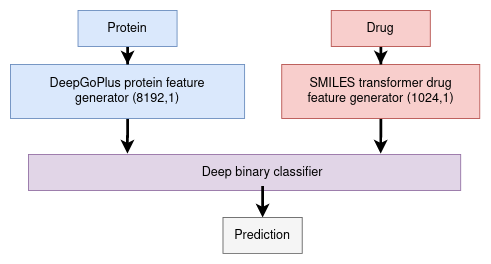
\includegraphics[width=0.4\textwidth]{figures/MolecularPredictor.png}}
	\caption{Molecular predictor based on the generated features from DeepGoPlus and SMILES transformer.}\label{fig:MolPred}
\end{figure}

\begin{figure}[!tpb]%figure2
\centerline{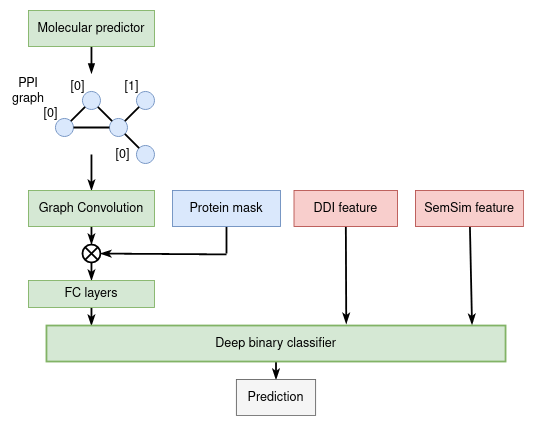
\includegraphics[width=0.4\textwidth]{figures/InteractionNetwork.png}}
\caption{Deep neural network that predicts based on drug-drug interaction features and semantic similarity features over side effects for drugs, and graph convolution over protein-protein interaction networks for proteins. Protein and drug features are represented by blue and red, respectively.}\label{fig:02}
\end{figure}

\section{Discussion}







%%%%%%%%%%%%%%%%%%%%%%%%%%%%%%%%%%%%%%%%%%%%%%%%%%%%%%%%%%%%%%%%%%%%%%%%%%%%%%%%%%%%%
%
%     please remove the " % " symbol from \centerline{\includegraphics{fig01.eps}}
%     as it may ignore the figures.
%
%%%%%%%%%%%%%%%%%%%%%%%%%%%%%%%%%%%%%%%%%%%%%%%%%%%%%%%%%%%%%%%%%%%%%%%%%%%%%%%%%%%%%%






\section{Conclusion}

\vspace*{-10pt}


\section*{Acknowledgements}

\vspace*{-12pt}

\section*{Funding}

This work has been supported by the... Text Text  Text Text.\vspace*{-12pt}

%\bibliographystyle{natbib}
%\bibliographystyle{achemnat}
%\bibliographystyle{plainnat}
%\bibliographystyle{abbrv}
%\bibliographystyle{bioinformatics}
%
%\bibliographystyle{plain}
%
\bibliography{citations}


\end{document}

%%% Local Variables:
%%% mode: latex
%%% TeX-master: t
%%% End:
